This chapter provides a deeper look into the implementation of the classifiers discussed in the above chapters.
The results of the data gathering process are also discussed here, with an evaluation of the classifiers' performance on the
portion of the dataset reserved for testing.
Finally, this chapter evaluates the classifiers' performance against real-world metrics and discusses their strengths and weaknesses.


\section{Sample gathering and dataset development}
\label{sec:sample-gathering-and-dataset-development}
The gathered dataset consisted of roughly two kilograms of roasted coffee, gathered
from two small-scale, specialty coffee roasters: Harmony Roasters based in York and Vibe
With coffee based in Nottingham.
Both roasters mentioned performing manual quality control
after every roast session and expressed interest in the automation of this process,
echoing the research aims of the project.

Between november and february 2023, both roasters were asked
to keep track of any defective beans they come across and separate the defects by
the variety the coffee belonged to.
Neither roaster asked for compensation for
their work, however, samples of non-defective beans were purchased for their usual
retail price, ensuring that the research process would not take any advantage of
their time and effort.

Upon gathering the beans, the defective beans were inspected once again with the defects separated.
The separation was done after a
consultation with the coffee roasters, who provided a verbal description of each
defect's visual characteristics.
The non-defective beans were also double-checked
for any defects in order to ensure the least amount of incorrectly labelled
samples.

To digitize the dataset, beans of each group were arranged in $5 \times 5$ grids
(where possible) and photographed using the main lens of a Pixel 7 pro smartphone.
All images were taken on a bright white background, with care taken to not include any dust or debris in the image.
Overhead lights along with a smaller tabletop light were used to make sure lighting levels stayed consistent between pictures.
Images of each defect were stored locally on the smartphone with backups made
in google images and GitHub.

Overall, the dataset contained 2786 images, each annotated with the bean variety,
the processing method used and the defect (or lack thereof) present in the bean.
To attempt to combat class imbalance, in cases where a bean
exhibited several defects at once, it was labelled as the rarer defect.
For
example, if the bean was both a ''quaker`` (underdeveloped) and had insect damage,
it was labelled as having insect damage only.
While not a perfect solution, this
ensured a satisfactory number of images per class.

\begin{figure}[h]
    \centering
    \begin{subfigure}
    {0.25\textwidth}
        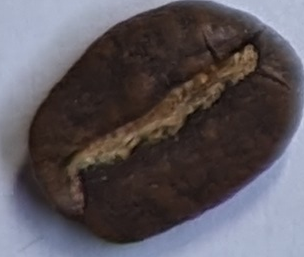
\includegraphics[height=0.8\linewidth, keepaspectratio]{
            ./figures/methodology/normal-bean
        }
        \subcaption{Normal} \label{fig:normalBeanSingle}
    \end{subfigure}
    \begin{subfigure}
    {0.25\textwidth}
        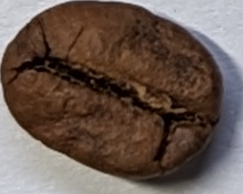
\includegraphics[height=0.8\linewidth, keepaspectratio]{
            ./figures/methodology/quaker-bean
        }
        \subcaption{''Quaker``} \label{fig:quakerBeanSingle}
    \end{subfigure}
    \begin{subfigure}
    {0.2\textwidth}
        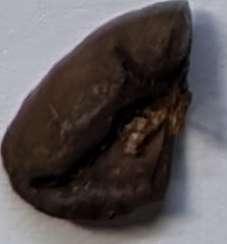
\includegraphics[width=0.8\linewidth, keepaspectratio, angle=270]{
            ./figures/methodology/bean-fragment
        }
        \subcaption{Bean \\ fragment} \label{fig:fragBeanSingle}
    \end{subfigure}
    \begin{subfigure}
    {0.2\textwidth}
        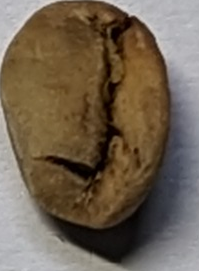
\includegraphics[width=0.8\linewidth, keepaspectratio, angle=90]{
            ./figures/methodology/under-bean
        }
        \subcaption{Underroasted} \label{fig:underBeanSingle}
    \end{subfigure}
    \begin{subfigure}
    {0.25\textwidth}
        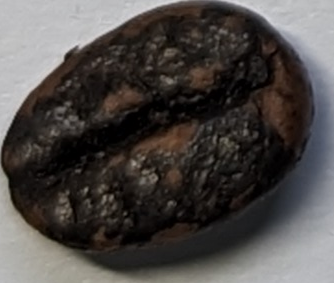
\includegraphics[height=0.8\linewidth, keepaspectratio]{
            ./figures/methodology/burnt-bean
        }
        \subcaption{Burnt} \label{fig:burntBeanSingle}
    \end{subfigure}
    \begin{subfigure}
    {0.2\textwidth}
        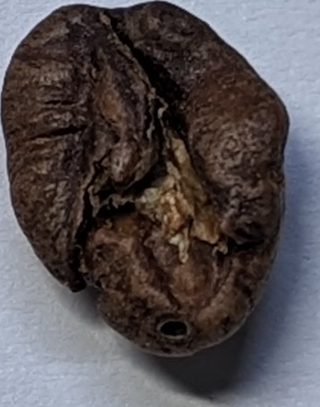
\includegraphics[height=0.8\linewidth, keepaspectratio]{
            ./figures/methodology/insect-damaged-bean
        }
        \subcaption{Insect \\ damage} \label{fig:insectBeanSingle}
    \end{subfigure}
    \begin{subfigure}
    {0.25\textwidth}
        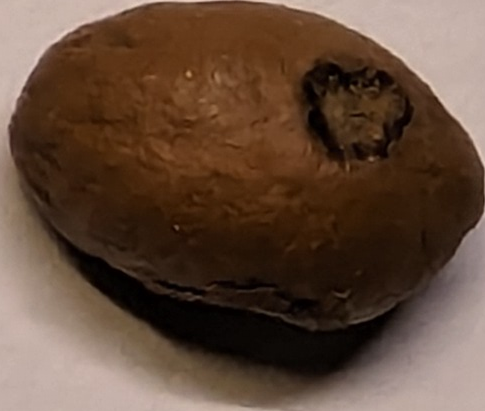
\includegraphics[height=0.8\linewidth, keepaspectratio]{
            ./figures/methodology/mold-damaged-bean
        }
        \subcaption{Mould damage} \label{fig:moldBeanSingle}
    \end{subfigure}
    \caption{Examples of bean defects}
    \label{fig:beanDefects}
\end{figure}

\begin{table}[h]
    \centering
    \begin{tabular}{p{0.2\textwidth}p{0.7\textwidth}p{0.1\textwidth}}
        \toprule \textbf{Defect name} & \textbf{Visual features}                                                                                   & \textbf{Count} \\
        \midrule Normal bean          & Even colour, brown to dark-brown hue, no surface damage or blemishes and a round shape with no deformities                                                           & 1311           \\
        Quaker & Light brown to brown hue (due to less caramelisation of sugar), scorch marks, brown spots on surface.
        Occasionally, a shrivelled, uneven look of the outside surface & 978            \\
        Bean fragment                 & Significantly deformed or chipped exterior, smaller bean pieces                                            & 296            \\
        Underroasted                  & Very light brown exterior, dark green or yellow in extremely underroasted beans                                                                                      & 104            \\
        Burnt                         & Dark brown to black exterior, significant scorching or an oily, shiny surface                                                                                        & 50             \\
        Insect/mould damage           & Small, round holes or larger ''craters`` on the surface                                                    & 47             \\
        \bottomrule
    \end{tabular}
    \caption{Bean defect counts}
    \label{tab:beanDefectCounts}
\end{table}
Overall, the beans exhibited five various defects, whose
counts and short descriptions are presented in table~\ref{tab:beanDefectCounts}.
Figure~\ref{fig:beanDefects} provides a brief look at the various defects.

The beans in the dataset belonged to a total of nine varieties and have been processed using six different methods.
The number of beans belonging to each processing method and variety method is shown
on figures~\ref{fig:beanProcessingCounts} and~\ref{fig:beanVarietyCounts} respectively.
\begin{figure}[h]
    \centering
    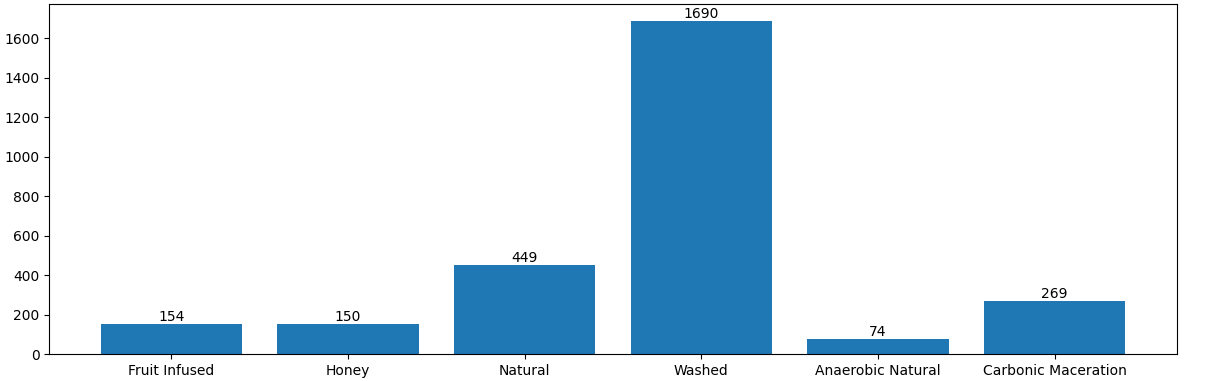
\includegraphics[width=\linewidth, height=2.5cm, keepaspectratio]{
        ./figures/methodology/processing-counts
    }
    \caption{Bean processing method counts}
    \label{fig:beanProcessingCounts}

    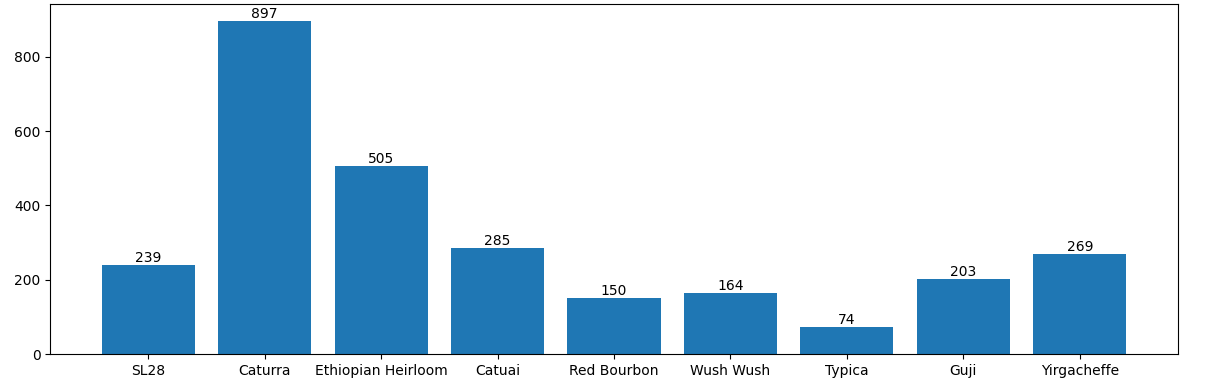
\includegraphics[width=\linewidth, height=2.5cm, keepaspectratio]{
        ./figures/methodology/variety-counts
    }
    \caption{Bean variety counts}
    \label{fig:beanVarietyCounts}
\end{figure}

It should be noted that the original intent was for the insect and mould damage to be distinct classes,
however, these defects are quite rare, especially with the higher-grade green coffee the local roasters worked with.
Therefore, it was decided to merge the classes: not only do the visual features of the two
defects resemble each other, but the effects they have on the final product are also similar.
While future work could seek an improved dataset and a higher granularity of classes, the merging of the two classes here
is unlikely to reduce the practical usefulness of the classifier in a roaster's daily tasks.

As described above, the beans were arranged in grids when their pictures were taken.
To train the classifier however, each bean had to be contained in its own image, requiring the use of a software solution
to automatically separate each bean.
The solution was implemented in Python and depended heavily on the OpenCV library~\cite{opencvLibrary}, which provides
tools for working with and processing images.

Separating the grid images involved several steps.
First, the image was loaded and converted to grayscale using a built-in OpenCV function.
Then, a threshold was applied to the resulting images to provide a binary separation between the beans and the background.
An important step was inverting the thresholded images so that the background was represented by black pixels
and the beans by white ones - this was required for the contour finding step that followed.

Once the binary images were produced, the \verb|findContours| function was used to identify the contours and
bounding rectangles of each individual bean.
At this stage, additional checks were conducted to ensure that no dust or foreign objects were captured by the algorithm:
bounding rectangles whose areas were uncharacteristically small or large or whose aspect ratio was too imbalanced were rejected.
The expected dimensions were gathered by running the algorithm once and inspecting the produced images: the images tended
to be around 200--400 pixels wide/tall, with an aspect ratio not exceeding 1:3.
Finally, the batch images were separated into sections matching the positions and dimensions of each bounding rectangle.
The resulting images were named reflecting the bean's variety, origin, processing method and defect class and sorted into folders
named in the same pattern.
A CSV file reflecting the class annotations has also been generated and stored in the image directory.
Each row in the CSV file corresponded to a single bean, with the columns containing the image name and the
aforementioned class information.

A visualisation of the data processing pipeline is shown on figure~\ref{fig:imgProcessing}.

\begin{figure}[h]
    \centering
    \begin{tikzpicture}
        \node (raw)
        {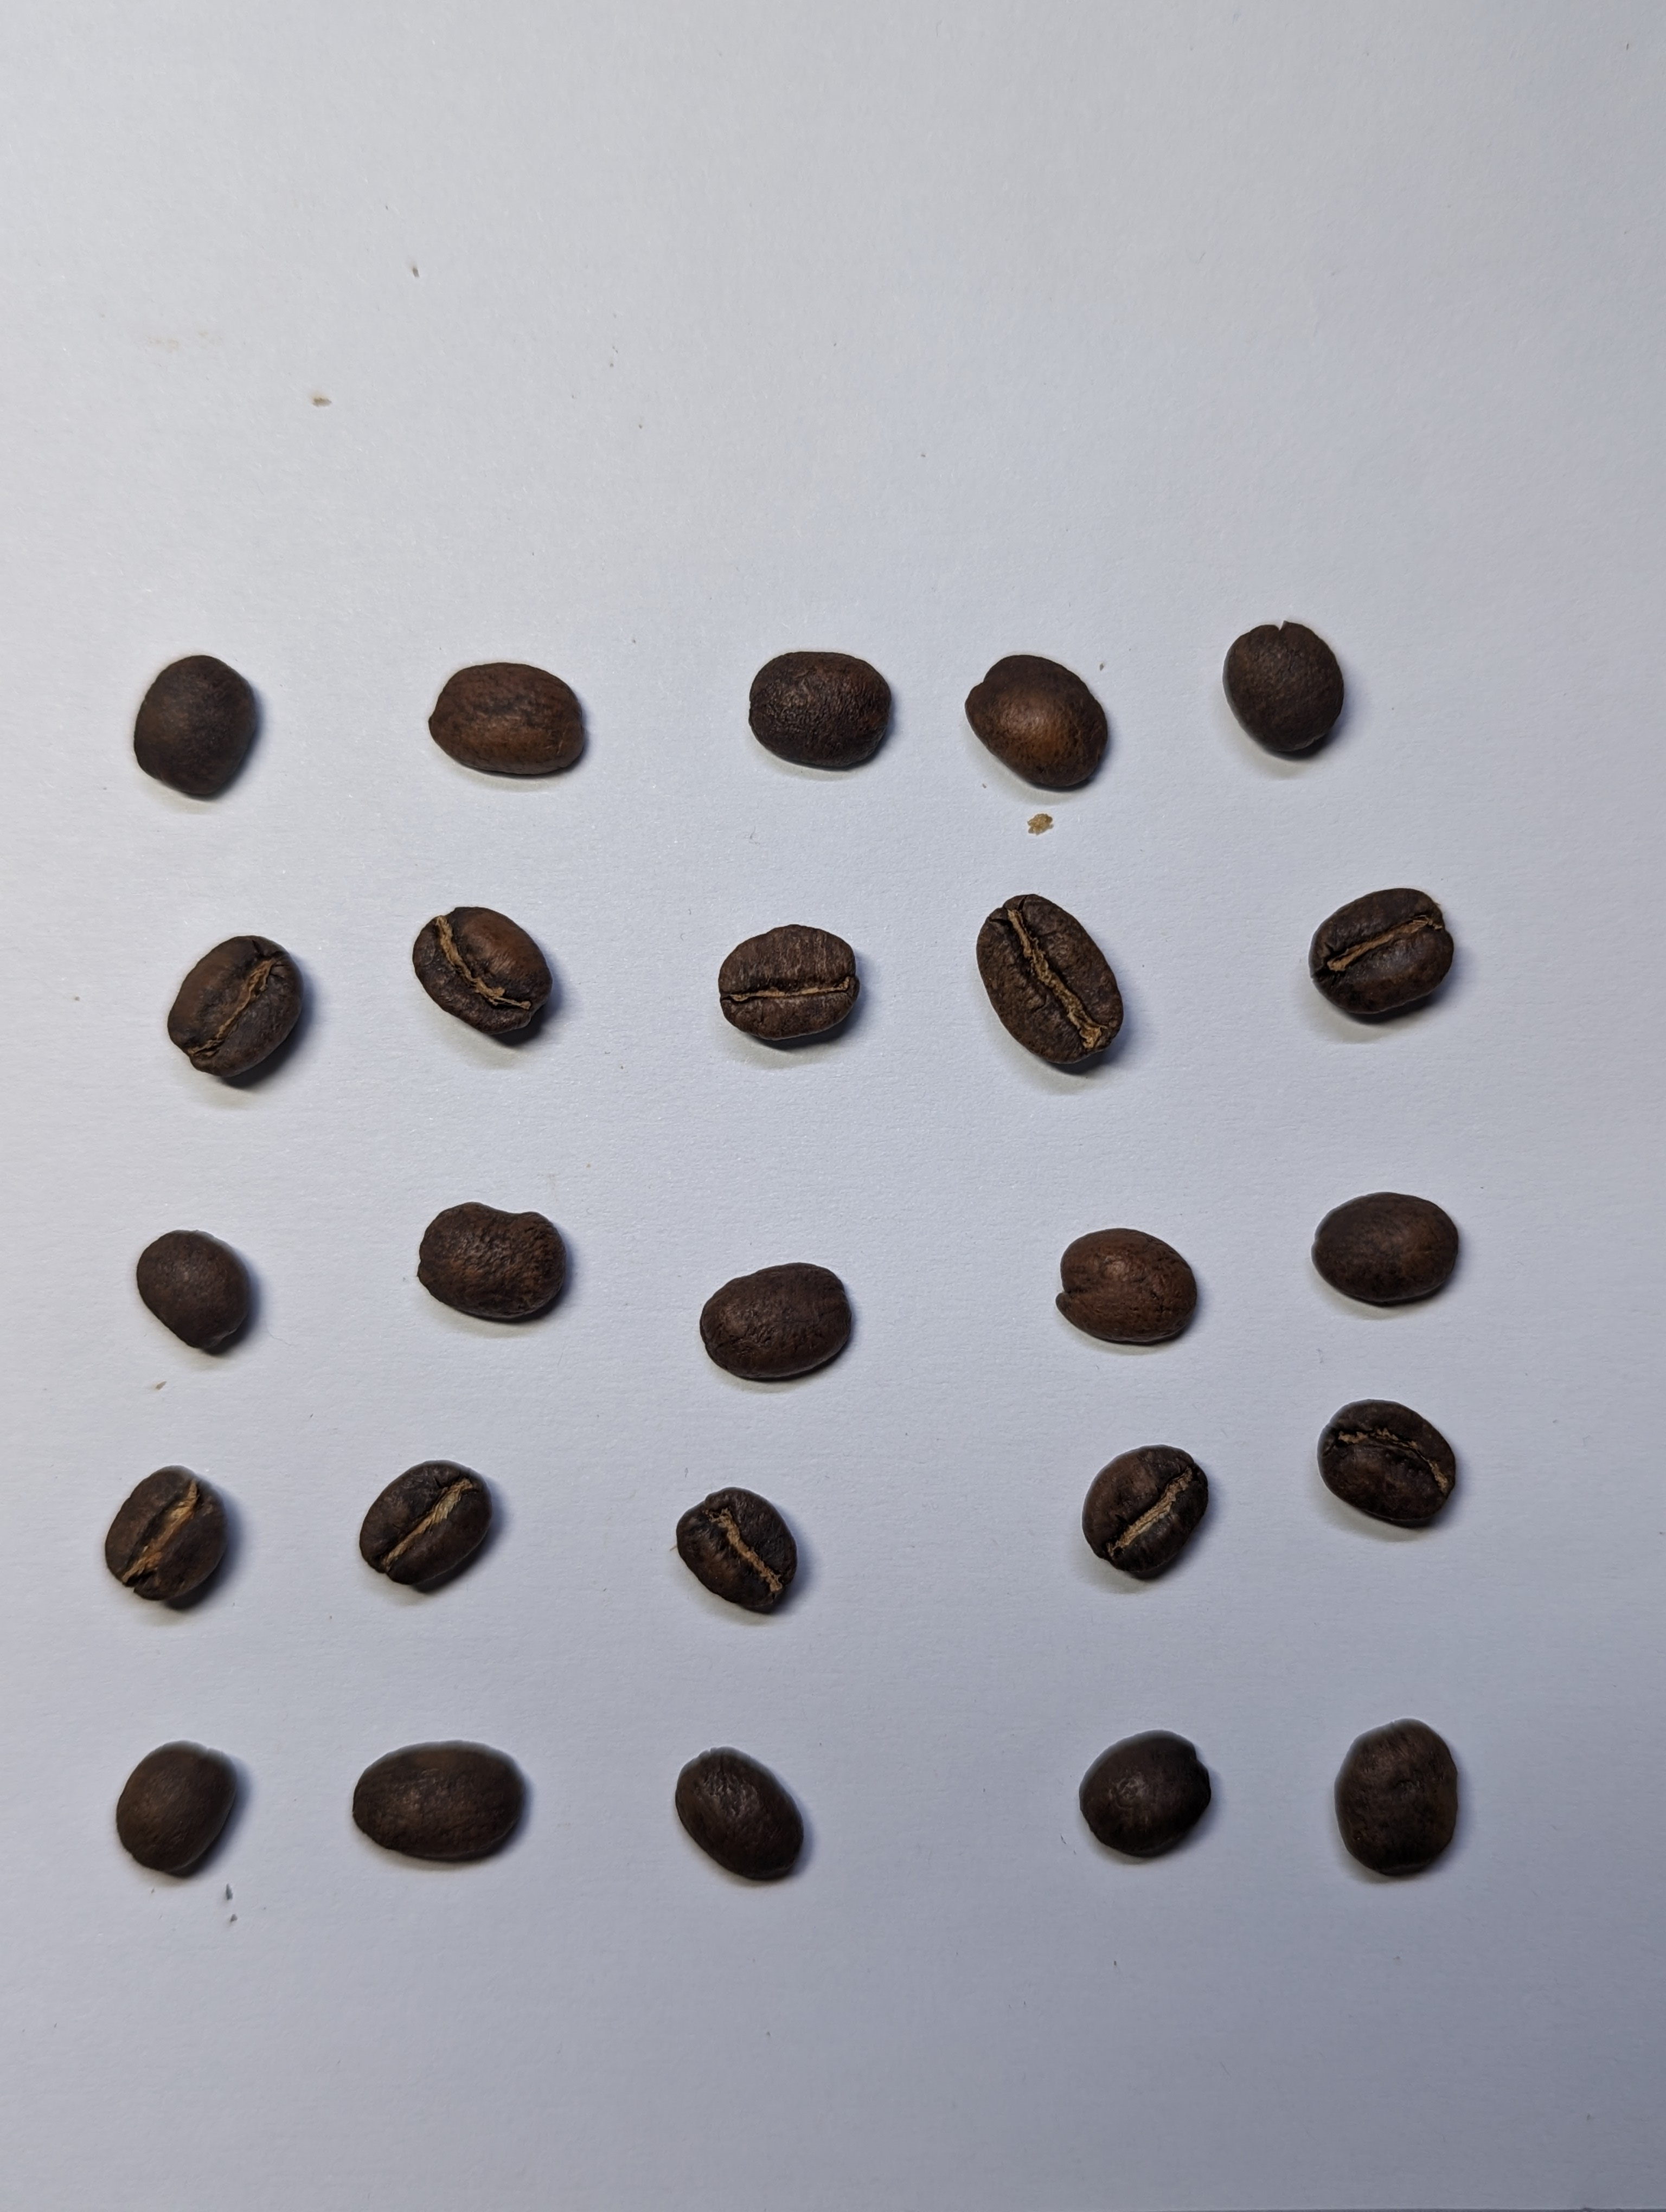
\includegraphics[height=3cm, keepaspectratio]{methodology/bean-batch-raw}};
        \node[right=of raw](gray)
        {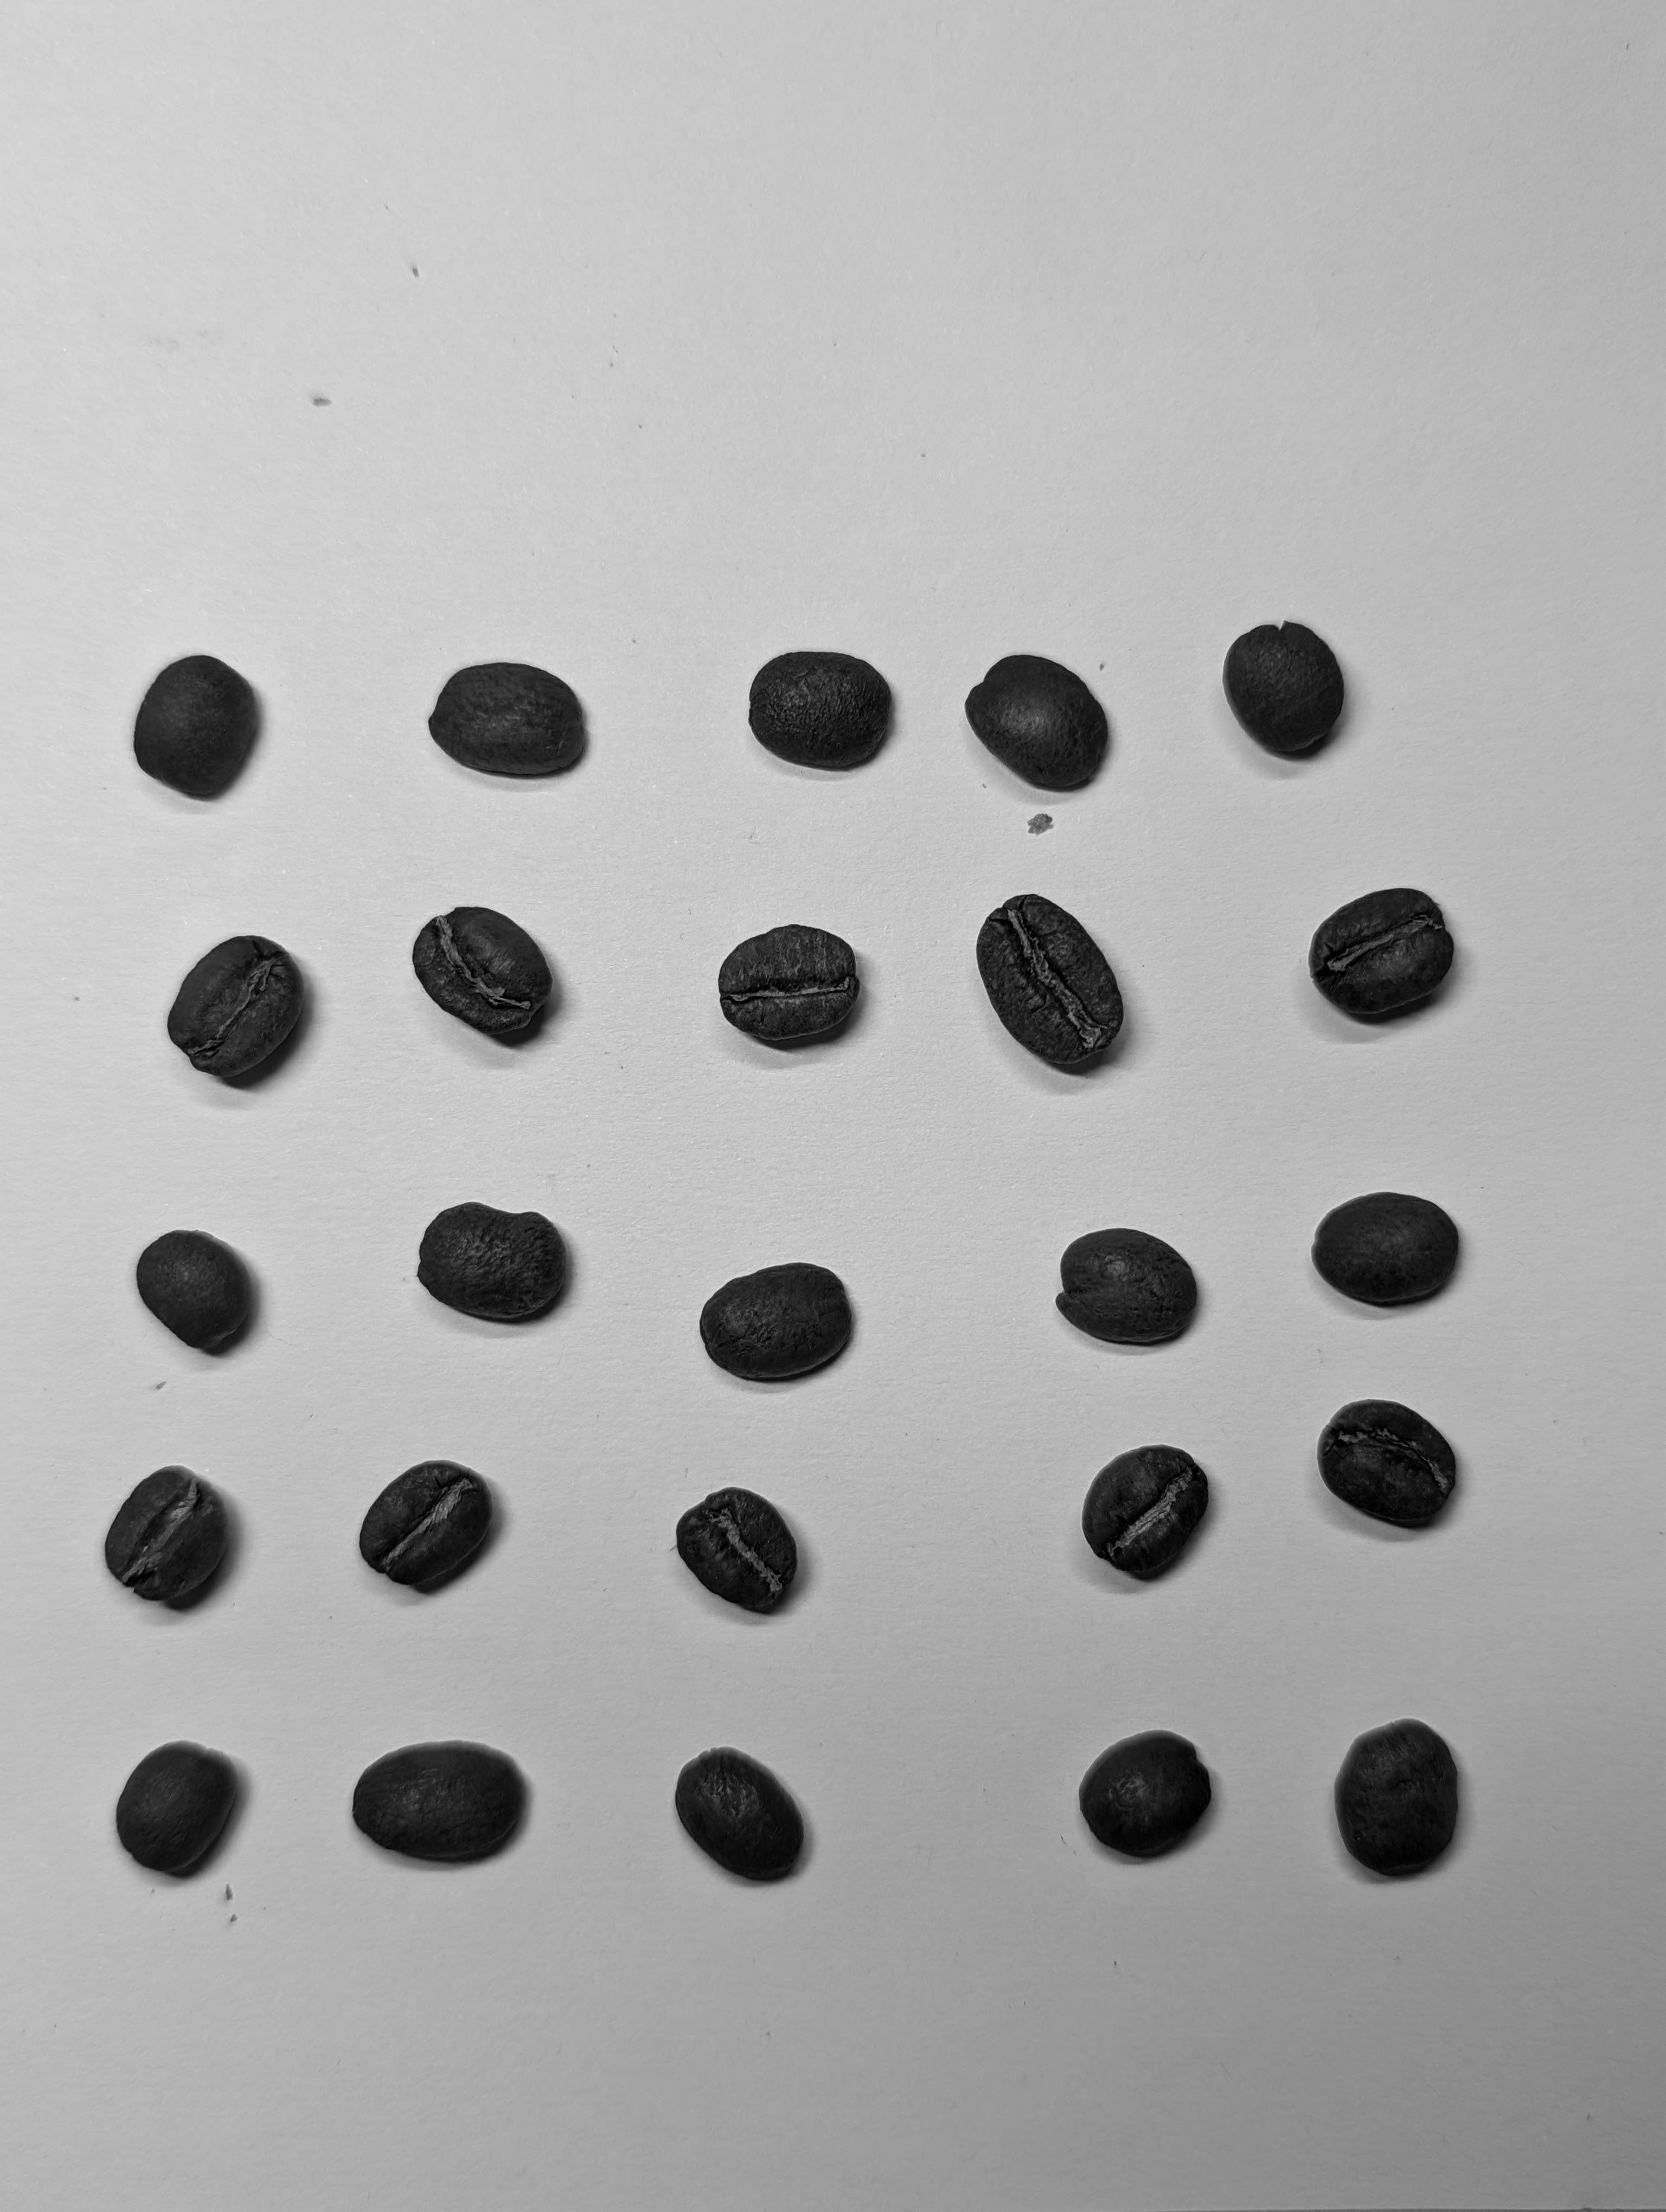
\includegraphics[height=3cm, keepaspectratio]{methodology/bean-batch-gray}};
        \node[right=of gray] (thresh)
        {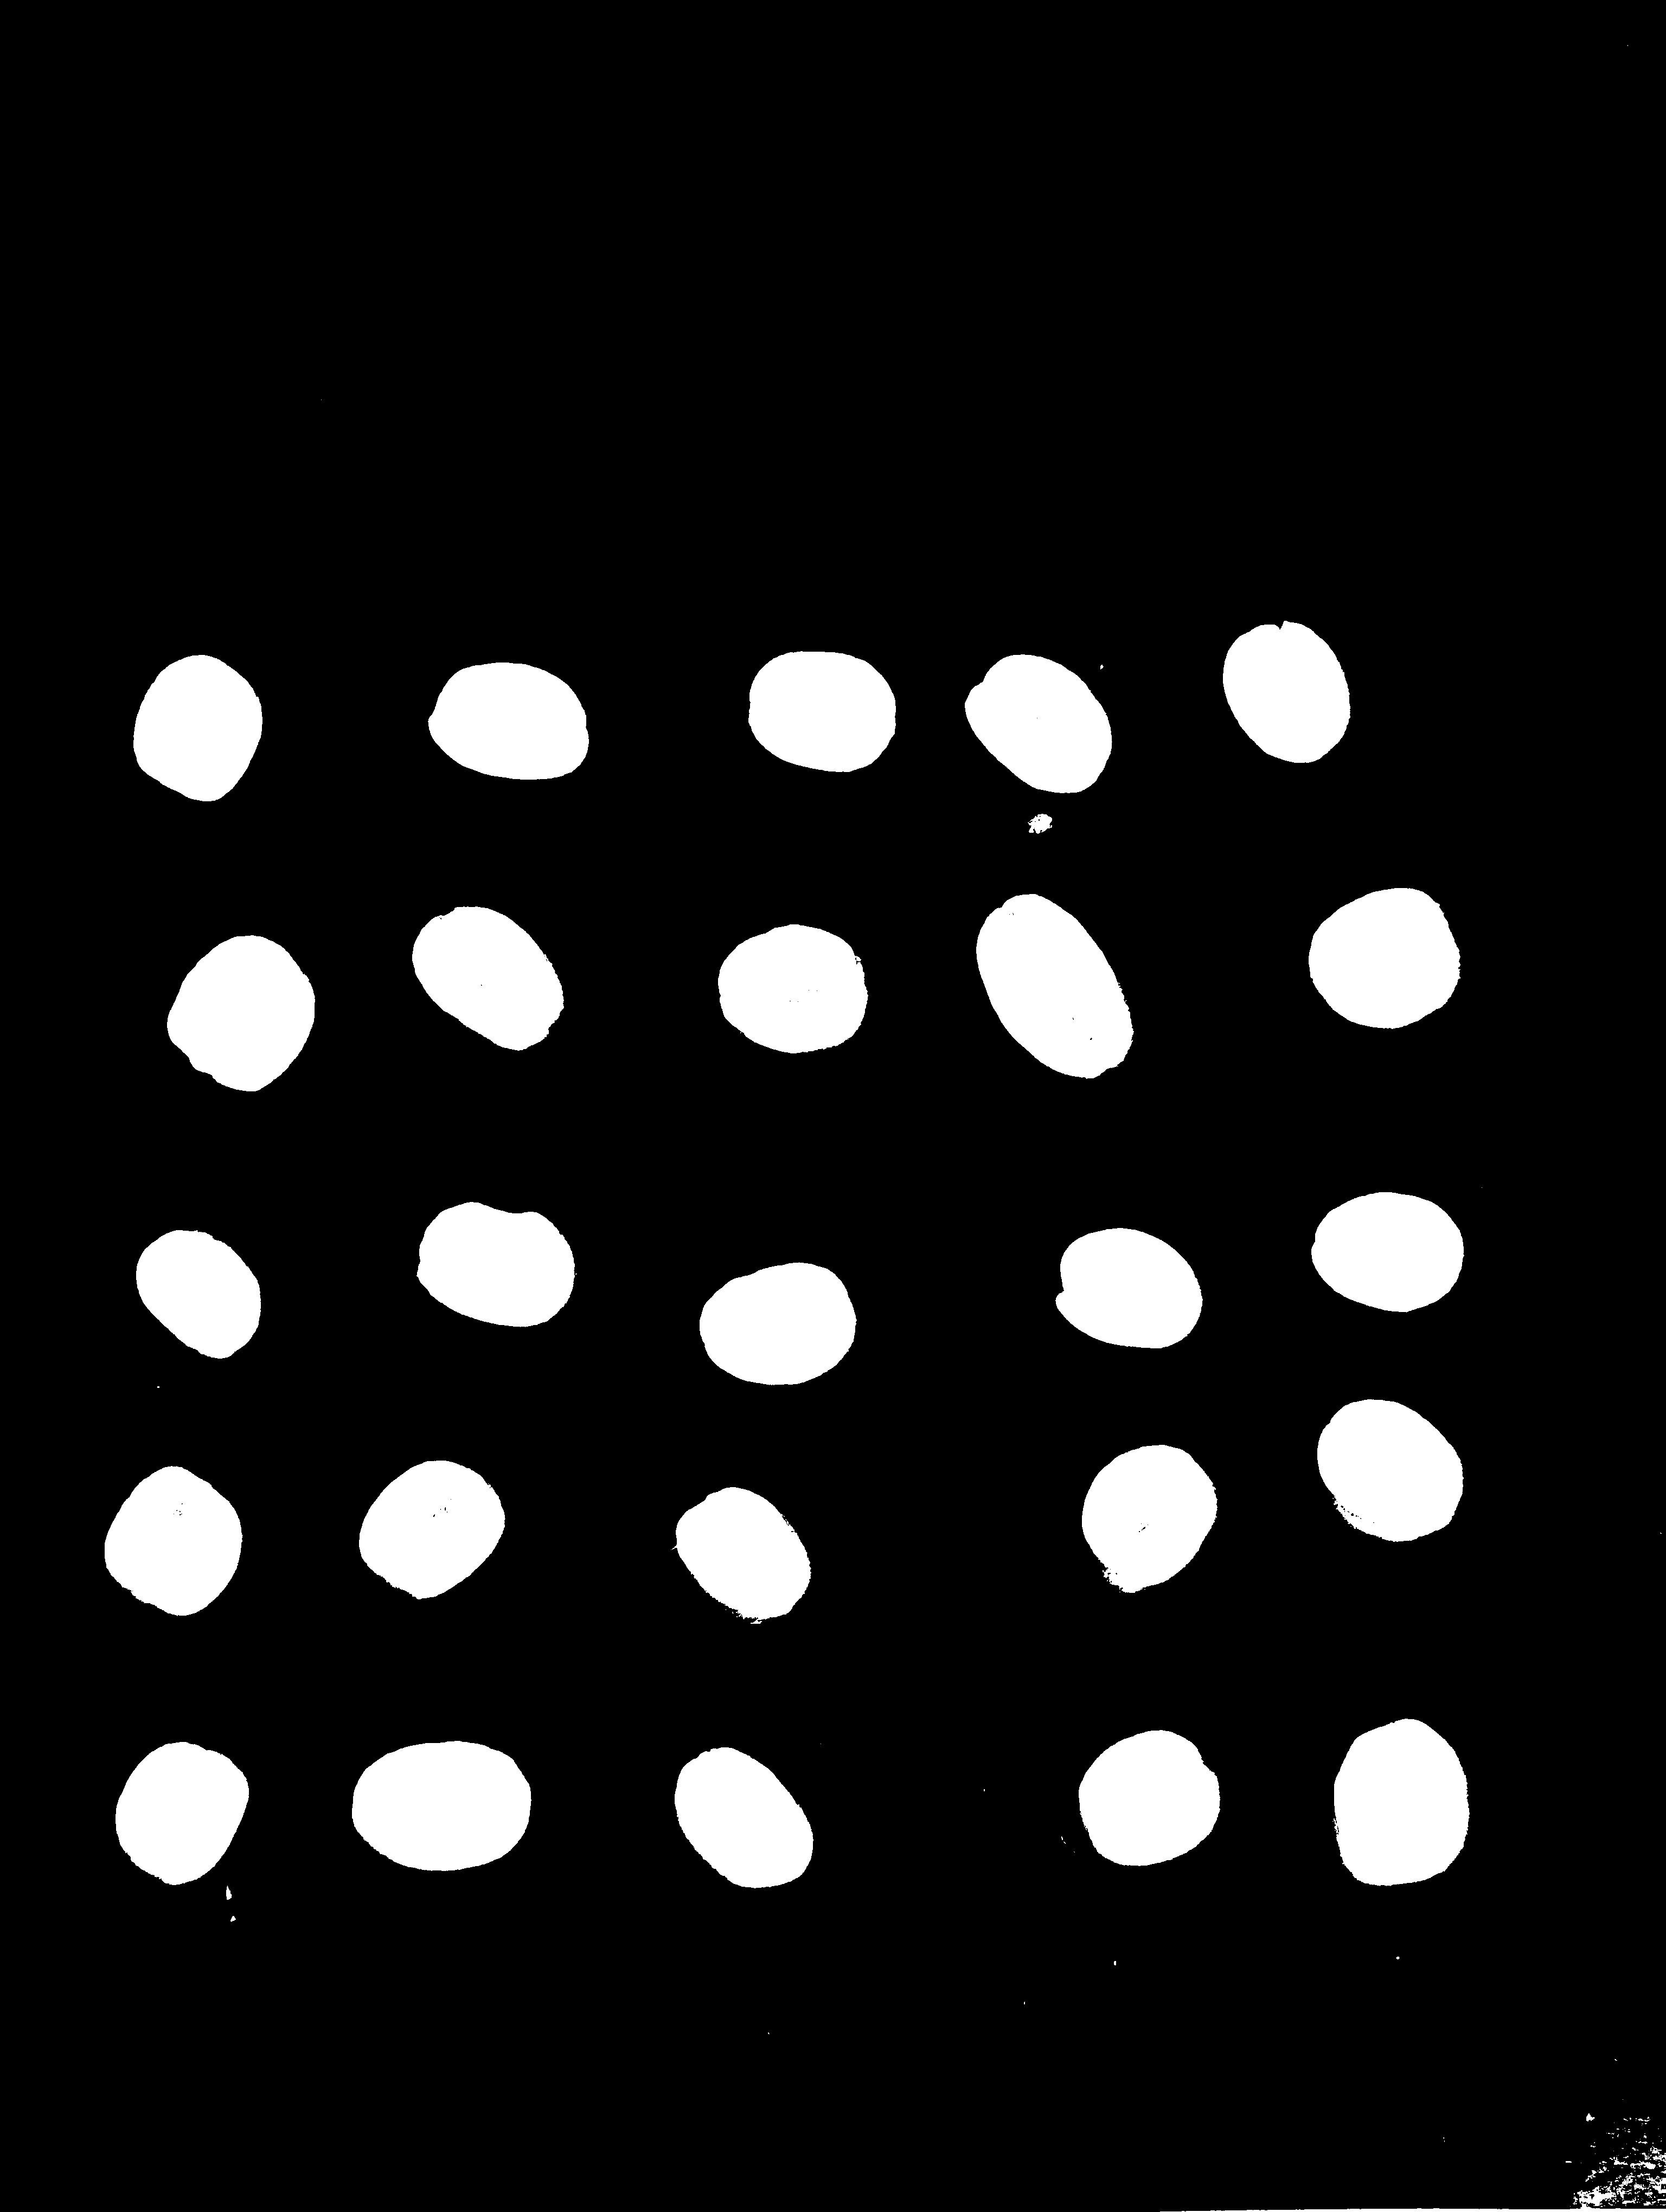
\includegraphics[height=3cm, keepaspectratio]{methodology/bean-batch-thresh}};
        \node[right=of thresh] (contours)
        {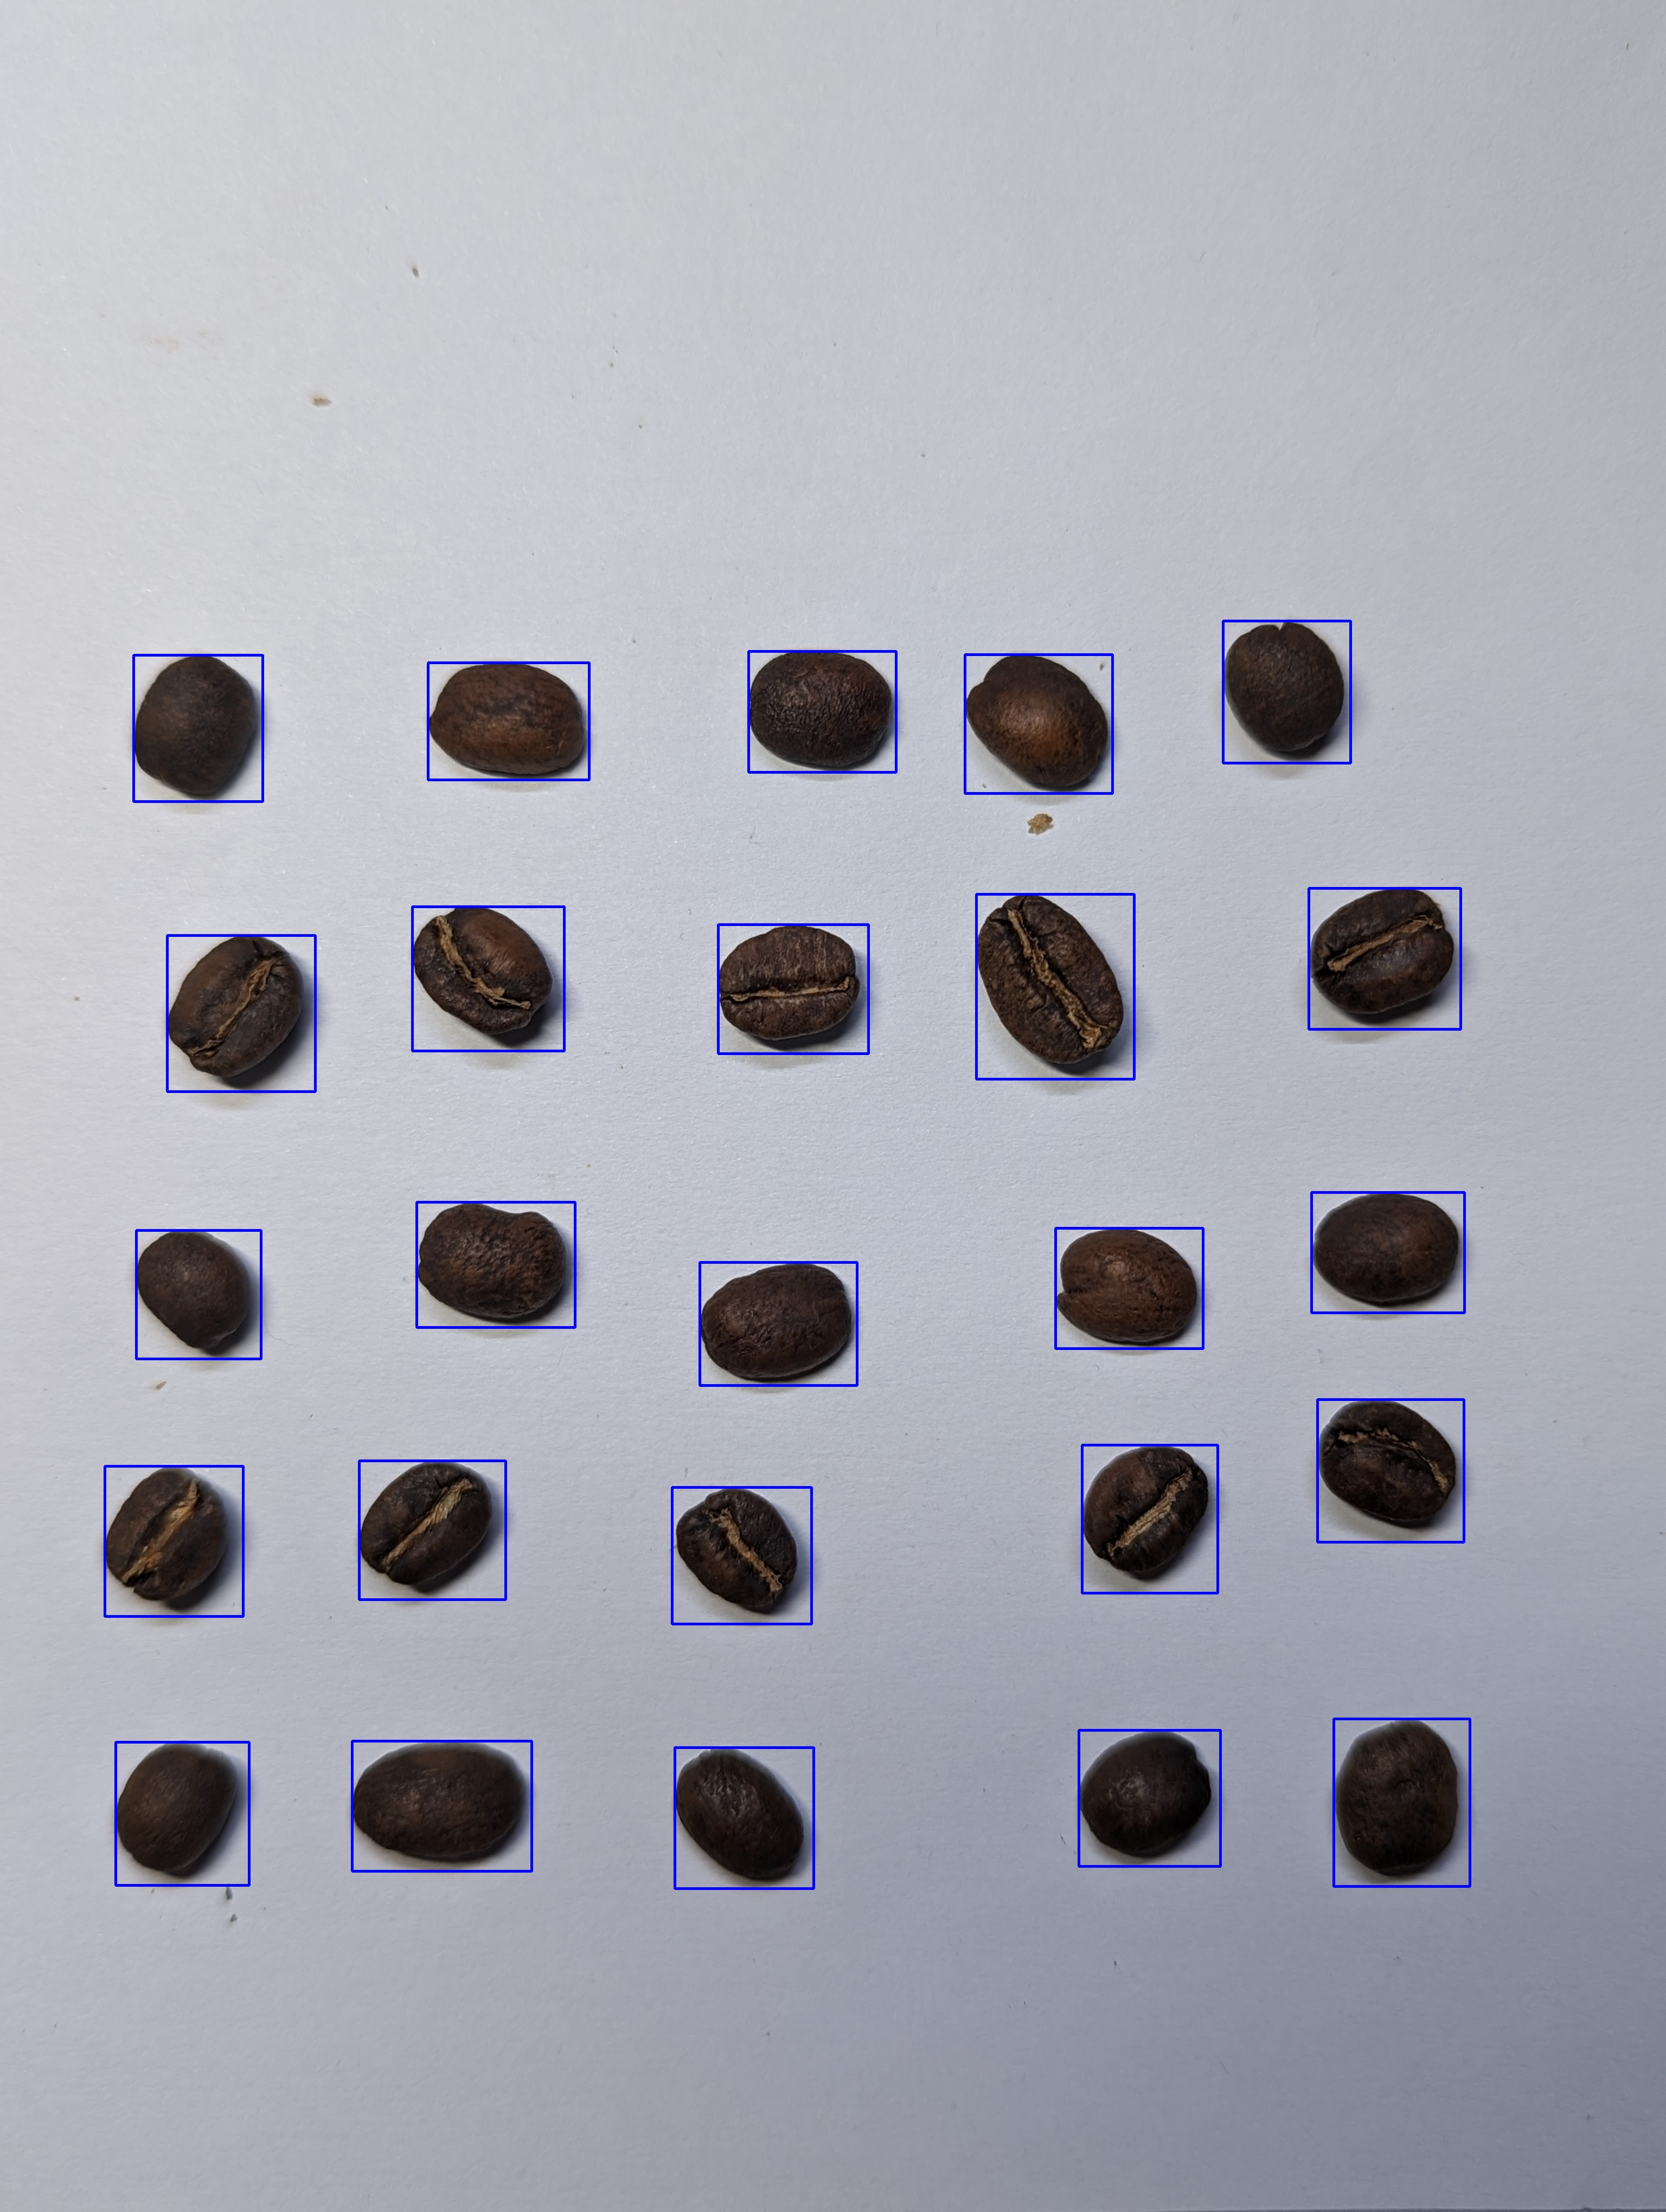
\includegraphics[height=3cm, keepaspectratio]{methodology/bean-batch-contours}};

        \draw[->,thick] (raw) -- (gray);
        \draw[->,thick] (gray) -- (thresh);
        \draw[->,thick] (thresh) -- (contours);
    \end{tikzpicture}
    \caption{Image processing pipeline}
    \label{fig:imgProcessing}
\end{figure}

It should be noted that preliminary experiments led to another addition to the image processing steps:
it was found that better performance was achieved when the natural background of the images was replaced with pure white pixels.
To achieve that, the thresholded images were used to manually set all non-bean (i.e. black) pixels to a value of (255, 255, 255),
resulting in a pure white background.
Both versions of the datasets were retained and used in classifier training.

Overall, the data processing pipeline yielded a dataset containing the individual images in a nested directory, with
a CSV annotations file in the top-level directory to be used by a machine learning framework.


\section{Loading and pre-processing the dataset}
\label{sec:loading-and-pre-processing-the-dataset}
Associating images with labels as well as final pre-processing and loading of the data was done by a PyTorch \verb|DataLoader|.
After the images were loaded, they were resized to the same $400 \times 400$ resolution, ensuring that most images are
enlarged rather than shrunk.
This was a conscious choice, as the textural features of some defects were quite small and harsh shrinking of the images
could have corrupted or outright removed that information.

After the images were set to a consistent size, the further processing differed slightly between the classifier types:
for the KNN classifier, no further processing was done.
This decision was based on the reasoning in section~\ref{sec:knn-classifier} and aimed to preserve the colour values of the pixels.
For neural network-based classifiers, the processing consisted from a sequence of transforms from the Pytorch \verb|torchvision.transforms|
package and consisted of the following items:
\begin{itemize}
    \item Converting the images to the \verb|float32| data type to enable training on the Apple Silicon M3 GPU cores
    \item For the training set, applying a random horizontal flip and a rotation to augment the dataset
    \item For the testing set, only applying a rotation to augment the test data due to its small size
\end{itemize}

After applying a stratified train/test split, with 80\% of images used for training, the class counts for the two sets are
shown in table~\ref{tab:finalTrainTestClassCuts}.
The split was applied with a constant random state value for repeatable results.
\begin{table}[h]
    \centering
    \begin{tabular}{lll}
        \toprule
        \textbf{Defect name} & \textbf{Training count} & \textbf{Testing count} \\
        \midrule
        Normal               & 1048                    & 263                    \\
        Quaker               & 782                     & 196                    \\
        Bean fragment        & 237                     & 59                     \\
        Underroasted         & 83                      & 21                     \\
        Burnt                & 40                      & 10                     \\
        Insect/Mould         & 38                      & 9                      \\
        \midrule
        \textbf{Total}       & 2228                    & 558                    \\
        \bottomrule
    \end{tabular}
    \caption{Finalised training and testing set class counts}
    \label{tab:finalTrainTestClassCuts}
\end{table}

As seen from the the above table, despite the initial aims of the project, the distribution of the classes was quite unbalanced.
While no ill effect on the KNN performance has been observed, such a skewed distribution is highly likely to negatively
affect the performance of a neural network due to the low chance of a smaller class' sample being picked in a given epoch.

While Pytorch provides facilities for sampling from a given list of indices and sampling with a manually set probability for each class,
there is no built-in method for combining the two, making it difficult to apply a weighted sampler to a subset of the total dataset.
The solution to this problem was found in a third-party library~\cite{imbalancedSampler} providing the \verb|ImbalancedDatasetSampler| class.
This sampler draws from a given list of indices with the probability of each class' sample being picked equal to
$P(Class_{sample} = C) = \frac{1}{\arrowvert\{x \in X \colon Class_x = C\}\arrowvert}$ for class $C$ and dataset $X$.

Overall, by combining the techniques of over and under sampling as well as data augmentation, the networks were able to learn on a relatively
evenly balanced and varied dataset.


\section{KNN classifier results}
\label{sec:knn-results}
The experiments with a KNN classifier followed the methods outlined in section~\ref{sec:knn-classifier}.
The sets of hyperparameters used to tune the classifier were as follows:
\begin{itemize}
    \item Distance calculation metric $M=\{Euclidean, Manhattan, Canberra\}$
    \item Number of nearest neighbours $K=[1, 30]$
    \item Nearest neighbour calculation algorithm $A=\{KDTree, Brute-force\}$
    \item Number of bins in colour histogram $N=\{32, 64, 128, 256\}$
\end{itemize}

All but the last hyperparameter were chosen via a grid search, with the number of bins being
set separately as it was applied to the dataset itself prior to fitting the classifier.

The experiments produced two noteworthy classifiers, whose hyperparameter choices and overall accuracy are presented in table~\ref{tab:knnResults}.
\pagebreak
\begin{table}[h]
    \centering
    \begin{tabular}{@{}lllll}
        \toprule
        & \textbf{\makecell{Distance \\metric}} & \textbf{K value} & \textbf{\makecell{Calculation \\algorithm}} & \textbf{\makecell{Histogram  \\bin count}} \\
        \midrule
        \textbf{KNN-1} & Manhattan  & 9  & KDTree & 32 \\
        \textbf{KNN-2} & Canberra  & 6  & KDTree & 256 \\
        \bottomrule
    \end{tabular}
    \caption{Finalised KNN classifiers}
    \label{tab:knnResults}
\end{table}

As seen from the above table, both classifiers achieved a relatively high accuracy.
However, inspecting the per-class performance of these classifiers reveals a significant difference.
A metric that can be used to compare per-class performance is the f1-score:
$f_1 = \frac{2tp}{2tp + fp + fn}$, where $tp$, $fp$ and $fn$ are the true positive, false positive and false negative rates respectively.
It should be noted that even the f1 score may not show the full picture: it may be insightful to also look at the precision
($\frac{tp}{tp + fp}$) and recall ($\frac{tp}{tp + fn}$) values per each class.
These metrics for KNN-1 and KNN-2 are presented in table~\ref{tab:knnScores}.
\begin{table}
    \centering
    \begin{tabular}{*7l}
        \toprule
        \textbf{Class} & \multicolumn{3}{c}{KNN-1} & \multicolumn{3}{c}{KNN-2} \\
        \midrule
        {}            & Precision & Recall & F1   & Precision & Recall & F1   \\
        Normal        & 0.81      & 0.95   & 0.87 & 0.80      & 0.96   & 0.87 \\
        Quaker        & 0.74      & 0.85   & 0.79 & 0.80      & 0.80   & 0.80 \\
        Bean fragment & 0.69      & 0.19   & 0.29 & 0.80      & 0.27   & 0.40 \\
        Underroasted  & 0.83      & 0.24   & 0.37 & 0.80      & 0.57   & 0.67 \\
        Burnt         & 1.00      & 0.20   & 0.33 & 0.57      & 0.40   & 0.47 \\
        Insect/Mould  & 0.00      & 0.00   & 0.00 & 1.00      & 0.33   & 0.50 \\
        \midrule
        \textbf{Overall accuracy} & \multicolumn{3}{c}{78.0\%} & \multicolumn{3}{c}{\textbf{79.7\%}} \\
        \bottomrule
    \end{tabular}
    \caption{KNN classifier evaluation metrics}
    \label{tab:knnScores}
\end{table}

The above data suggests that the canberra distance metric allows the classifier to gain better
performance with the under-represented classes, while slightly reducing the performance on larger ones.
This is an important insight, suggesting that the metric can be picked according to the classifier's use case:
the manhattan metric can provide a powerful sorter where one may only be concerned from separating defective and normal beans,
while the canberra metric can provide insights into the distribution of the defects themselves.
It is clear, however, that the colour histogram may not be a powerful enough technique to explain the differences between
the defects and that a more sophisticated solution may be needed if an understanding of defect frequencies (or, an even more accurate sorter)
is the goal.


\section{Compact CNN results}
\label{sec:compact-cnn-results}
Similar to the above section, several model architectures have been tested.
Unlike with KNN classifiers, the hyperparameter space for neural networks is much greater, with many options of loss functions,
optimizer algorithms and more.
This meant that a simple grid search would be incredibly time and resource intensive and that a more thoughtful approach was needed.

The first item considered was the optimizer selection, with the Adam~\cite{adamGrad} and Stochastic gradient descent (SGD) algorithms being
the main candidates due to their wide adoption in industry and strong results on existing datasets.
While both optimizers showed good results when training the models, the SGD optimizer was chosen in the end for its ability
to be customized with momentum (with a value of 0.9 used) and its more intuitive operation.
With momentum, the optimizer updates the weights each epoch the following way:
$\theta_{t+1}=\theta_{t} - \gamma\nabla{f(\theta_{t})}+\mu\Delta\theta$, where $\gamma$ is the learning rate (set to 0.001),
$\mu$ is the momentum value and $\Delta\theta$ is the previous update of the weight vector $\theta$.

A loss function needed to be picked next - being a classification problem with multiple classes, binary methods were not applicable,
therefore the choice fell on the cross-entropy function, which at a high level, measures the extent to which the
probability distribution of the model's prediction matches that of the actual data.
It should be noted that the Pytorch implementation of this loss function differs slightly from the commonly seen definition,
requiring that the input to the loss function consists of the ''unnormalised logits for each class`` and the target is the class labels.
The overall function can be defined by $-\log{\frac{\exp(x_{n, y_{n}})}{\sum_{c=1}^C\exp(x_{n, c})}}$,
with each minibatch's loss being the average of the loss for each input~\cite{pytorchLibrary}.

Finally, the batch size and epoch number were selected experimentally - initial attempts showed a significant boost in accuracy
(though, at the expense of longer training times) when a smaller batch size was used: switching from 32 down to 4 led
to the biggest increase, with little to no gain seen from further reductions.
The number of epochs was determined from the size of the batches and from observing the magnitude of the changes in the loss function
with the optimal number being 40 for the shuffleNet and mobileNet architectures.

The optimal learning rate for the optimizer was different depending on the number of the current epoch.
While larger ''jumps`` were acceptable and even welcome at the earlier stages, a large learning rate could ruin tens of epochs
of training nearing the end of the training loop.
Therefore, instead of attempting to pick a single learning rate value, a scheduler provided by PyTorch was used.
The chosen solution was an instance of the \verb|StepLR| class, halving the learning rate every 10 epochs for both
ShuffleNet and MobileNet.
Overall, the two selected architectures achieved a significant improvement in both overall accuracy and per-class
metrics over the KNN classifier, with the results presented in table~\ref{tab:cnn-small-scores}.

\begin{table}
    \centering
    \begin{tabular}{*7l}
        \toprule
        \textbf{Class} & \multicolumn{3}{c}{MobileNet V2} & \multicolumn{3}{c}{ShuffleNet} \\
        \midrule
        {}            & Precision & Recall & F1   & Precision & Recall & F1   \\
        Normal        & 0.93      & 0.95   & 0.94 & 0.92      & 0.94   & 0.93 \\
        Quaker        & 0.77      & 0.90   & 0.83 & 0.82      & 0.75   & 0.78 \\
        Bean fragment & 0.93      & 0.50   & 0.64 & 0.77      & 0.63   & 0.69 \\
        Underroasted  & 0.57      & 0.62   & 0.60 & 0.28      & 0.76   & 0.41 \\
        Burnt         & 1.00      & 0.40   & 0.57 & 0.75      & 0.30   & 0.43 \\
        Insect/Mould  & 0.50      & 0.11   & 0.20 & 0.00      & 0.00   & 0.00 \\
        \midrule
        \textbf{Overall accuracy} & \multicolumn{3}{c}{\textbf{84\%}} & \multicolumn{3}{c}{81\%} \\
        \bottomrule
    \end{tabular}
    \caption{Compact CNN evaluation metrics}
    \label{tab:cnn-small-scores}
\end{table}

Overall, moving to a compact CNN has shown a great improvement in both accuracy and per-class metrics over the KNN
classifier.
Despite that, the performance in smaller classes is still somewhat lacking, with the underroasted, burnt and insect damaged
beans being frequently misclassified.
It is clear that the network is lacking information to build a knowledge of the features of these beans from the small
data samples the dataset provides.
The next section will look at addressing these shortcomings by applying transfer learning to a much larger model.


\section{Transfer learning results}
\label{sec:transfer-learning-results}
When selecting the models here, much less concern was given to the size of the model - the main criteria instead were
their performance on a known dataset like ImageNet~\cite{imageNet}.

The ResNet architecture stood out as having great performance on the dataset and a good track record of successful
transfer learning applications.
Several versions of the architecture exist, with 18, 34, 50 and 152 layers.
The first three were selected for experiments, with the extremely large size of the 152 layer version leading to excessively long
training loops and marginal gains over the smaller architectures in preliminary experiments.
For comparison, the MobileNet architecture from the previous section and Swin transformer~\cite{swinTransformer} were also trained,
with the latter serving as an example of a transformer network.

As mentioned in section~\ref{sec:transfer-learning}, each network was adjusted to predict 6 classes and trained using a similar
iterative approach as described in section~\ref{sec:compact-cnn-results}.

While training the models, it was discovered that they benefited from a higher initial learning rate of 0.01 and more aggressive scheduling,
with the ResNet models performing best with the learning rate reduced by ten times every eight epochs.
The best performing optimizer and loss function were SGD and Cross entropy loss respectively.

It should be noted that MobileNet and ResNet were trained entirely - that is, every weight was updated during training.
The Swin transformer on the other hand, had all its weights frozen (by marking them as not requiring gradient calculations in PyTorch)
except those in the final layer.
This was done as the extreme size of the Swin transformer network caused poorer performance on the smaller classes when all weights were updated -
retaining the weights trained on ImageNet allowed it to better classify the smaller bean categories.

\begin{table}[h]
    \centering
    \begin{tabular}{*{10}l}
        \toprule
        \textbf{Class} & \multicolumn{3}{c}{ResNet 18} & \multicolumn{3}{c}{ResNet 34} & \multicolumn{3}{c}{ResNet 50} \\
        \midrule
        {}     & {Prec.} & {Rec.} & F1   & {Prec.} & {Rec.} & F1   & {Prec.} & {Rec.} & F1   \\
        Normal & 0.93    & 0.98   & 0.96 & 0.96    & 0.99   & 0.98 & 0.99    & 0.99   & 0.99 \\
        \addlinespace[0.5em]
        Quaker & 0.93    & 0.89   & 0.91 & 0.94    & 0.92   & 0.93 & 0.95    & 0.92   & 0.94 \\
        \addlinespace[0.5em]
        \makecell[l]{Bean \\fragment} & 0.90 & 0.90 & 0.90 & 0.88 & 0.83 & 0.85 & 0.94 & 0.86 & 0.90 \\
        \addlinespace[0.5em]
        \makecell[l]{Under  \\roasted} & 0.80 & 0.76 & 0.78 & 0.77 & 0.81 & 0.79 & 0.60 & 1.00 & 0.75 \\
        \addlinespace[0.5em]
        Burnt & 0.86 & 0.60 & 0.57 & 1.00 & 0.60 & 0.75 & 0.91 & 1.00 & 0.95 \\
        \addlinespace[0.5em]
        \makecell[l]{Insect/ \\mould} & 0.83 & 0.56 & 0.67 & 0.67 & 0.89 & 0.76 & 1.00 & 0.67 & 0.80 \\
        \midrule
        \textbf{\makecell[l]{Overall \\accuracy}} & \multicolumn{3}{c}{92\%} & \multicolumn{3}{c}{94\%} & \multicolumn{3}{c}{\textbf{95.2\%}} \\
        \bottomrule
    \end{tabular}
    \caption{ResNet architecture evaluation metrics}
    \label{tab:resnet-scores}
\end{table}

Overall, the ResNet and MobileNet architectures showed the best results, with the 50 layer version achieving the best accuracy, though at the cost of a slightly longer
training time.
The best results were achieved on the white-background dataset (as described in section~\ref{sec:sample-gathering-and-dataset-development}),
with the per-class accuracy metrics presented in table~\ref{tab:resnet-scores}.
The same metrics for the pre-trained MobileNet and Swin transformer networks are displayed in table~\ref{tab:transfer-results-2}.

\begin{table}[h]
    \centering
    \begin{tabular}{*7l}
        \toprule
        \textbf{Class} & \multicolumn{3}{c}{MobileNet (pre-trained)} & \multicolumn{3}{c}{Swin transformer} \\
        \midrule
        {}            & Precision & Recall & F1   & Precision & Recall & F1   \\
        Normal        & 0.97      & 0.98   & 0.98 & 0.88      & 0.95   & 0.91 \\
        Quaker        & 0.95      & 0.97   & 0.96 & 0.79      & 0.87   & 0.83 \\
        Bean fragment & 0.91      & 0.85   & 0.88 & 0.86      & 0.71   & 0.78 \\
        Underroasted  & 1.00      & 0.90   & 0.95 & 1.00      & 0.19   & 0.32 \\
        Burnt         & 0.89      & 0.80   & 0.84 & 0.00      & 0.00   & 0.00 \\
        Insect/Mould  & 1.00      & 0.67   & 0.80 & 0.75      & 0.33   & 0.46 \\
        \midrule
        \textbf{Overall accuracy} & \multicolumn{3}{c}{\textbf{95.3\%}} & \multicolumn{3}{c}{85\%} \\
        \bottomrule
    \end{tabular}
    \caption{ResNet alternatives evaluation metrics}
    \label{tab:transfer-results-2}
\end{table}
Except the Swin transformer, the application of transfer learning brought significant improvements in
under-represented class performance as well as further increases in overall accuracy.
The confusion matrices for all classifiers discussed here are available in appendix~\ref{ch:appendix2}, while
the hyperparameter search results are available in appendix~\ref{ch:appendix3}.
The next section will discuss the real-world application potential of each of the classifiers.

\section{Evaluation}
\label{sec:evaluation}
While the high accuracy of the classifiers developed during the project makes a relatively strong case for it being a success,
it is still important to take a deeper look at the weaknesses and imperfections that might affect their usefulness in the industry.

First, it is important to consider the impact each defect has on the finished product: while both coffee roasters whose
samples were used in the project agreed that a defect-free product is the ultimate goal, they mentioned placing much more
effort and attention into removing quaker and insect/mould damaged beans than other defects.
This is due to the fact that while under and over-roasted coffee beans do affect the flavour of the cup, they do not
do so to nearly the same extent.
In other words, a small number of beans with no defects other than a wrong roast level is unlikely to damage their company's
reputation or economic prospects.

Second, the success criteria for a classifier can differ depending on the user's own goals - while some may only look for
a separation between normal and defective classes, others may wish for more thorough statistics on their product, with
the latter audience paying more attention to the model's performance in every class.

In any case, a balance of precision, recall and accuracy for the ''Normal`` class are equally
important for a classifier's viability: while an imprecise model will fail to identify normal beans leading to
a waste of good product and a negative impact on the finances of a roaster, a model with poor recall will mark too many
defective beans as normal, affecting the quality of the resulting product and the roaster's marketing potential.
With this in mind, the three kinds of models developed here can be evaluated.

The KNN classifier's performance leaves a lot to be desired - while KNN-1 achieved a good recall score for the ''Normal``
class, its precision is relatively low: a batch of coffee processed using this classifier will likely be sorted too agressively
with many good beans needlessly discarded.
Furthermore, the performance on smaller classes is quite poor, with only the ''Quaker`` classes achieving an F1 score above
0.5.
Despite this, the KNN approach still has its strengths, which mainly relate to its simplicity and transparency -
the general principle behind it is likely to be understood even by a non-technical audience and the dimensionality reduction
method is relatively straightforward and relies on simple observations of the beans.
While using a highly optimised algorithm such as the one implemented in Scikit-learn~\cite{sklearnLibrary} can dramatically reduce the resources
needed for a single prediction, calculating the colour histogram takes a much larger amount of time.
Furthermore, the prediction time is dependent on the size of the dataset, leading to slower prediction times as the dataset grows.

Switching to a simple neural network architecture results in a much more viable model: with the MobileNet architecture
being the best performer in that category, the precision and recall scores for the ''Normal`` class could potentially allow it
to be used in industry, similarly to its performance with the ''Quaker`` class.
On the testing set, the model displayed a good result, with its relatively low rate of normal beans classified as defective
making it highly useful as, for example, a first-stage sorter before a second, manual pass, greatly reducing the labour
needed to sort a batch of beans.

Finally, transfer learning produced the most versatile and high-performing models, with the ResNet and MobileNet achieving
quite similar results despite their significant size difference.
It can be said that the knowledge gained from a large general-purpose dataset transfers well to this relatively niche
application area, with the MobileNet's gain in identifying underrepresented classes being clear proof of this hypothesis.
This improvement in performance likely comes from the convolution layers' ability to develop filters that assess both the texture
and colour of the images, allowing the CNN models to better inform their classification.
The impact of that additional information on performance can be seen in examples shown in appendix~\ref{ch:appendix1}.
It should be noted that some examples in the appendix reveal a need for improved lighting and potentially, higher resolution images,
identifying one area of further work.
The use of transfer learning also reduced the amount of time needed for training, with both models requiring fewer epochs and less than an hour of training time.
Overall, the high performance, especially on larger classes, suggest a great potential of this approach
on a larger, more varied and balanced dataset.
To judge the models' performance as a sorting assistant, their error statics are presented on
figure~\ref{fig:real-world-scores}.

\begin{figure}
    \centering
    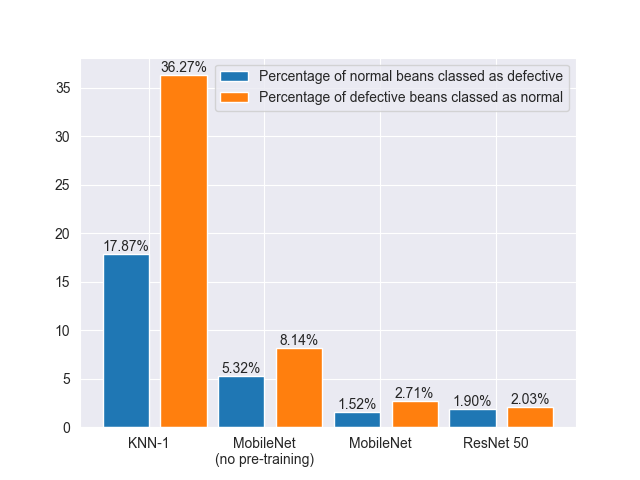
\includegraphics[width=\textwidth]{results/best-performers-results}
    \caption{Real-world application results for best performers}
    \label{fig:real-world-scores}
\end{figure}
From the above figure, it is evident that neural networks vastly outperform the KNN classifier,
\begin{wraptable}{r}{0.35\textwidth}
    \centering
    \begin{tabular}{lc}
        \toprule
        \textbf{Model} & \textbf{\makecell{Prediction \\time (ms)}}          \\
        \midrule
        KNN-2      & 8.32                        \\
        MobileNet      & 10.44                        \\
        ResNet 50      & 20.34                        \\
        \bottomrule
    \end{tabular}
    \caption{Average prediction time per bean (ms)}
    \label{tab:execTimes}
\end{wraptable}
with pre-training greatly reducing the waste of normal beans and the chance of a defective bean,
especially one with a high-impact defect, making it into the final product.
Overall, the pre-trained MobileNet architecture stands out as the best compromise between prediction time, accuracy and
real-world utility, with its prediction time (shown in table~\ref{tab:execTimes}) potentially allowing it to be used in real-time systems.
The ResNet architecture, could be of great use in environments where the importance of peak accuracy outweighs that of the
system's speed, such as when analysing a sample taken from a larger batch before agreeing on its purchase.

Overall, the dataset and models developed in this project show good potential of achieving the success criteria outlined
in section~\ref{sec:research-aims}: the dataset was developed entirely from scratch and showcases a range of origins and
processing methods that is reflective of the products offered by modern coffee roasters today.
The models' training was entirely achievable on consumer-grade hardware and took a reasonable amount of time to complete,
enabling roasters to quickly train their own models or instantly begin classifying by downloading the model weights developed here.



